\documentclass{article}

\PassOptionsToPackage{numbers,sort&compress}{natbib}
\usepackage[dblblindworkshop]{neurips_2026}
\workshoptitle{NEmo 2026: Neuro-Symbolic Embodied Intelligence}

\usepackage[utf8]{inputenc}
\usepackage[T1]{fontenc}
\usepackage{hyperref}
\hypersetup{hidelinks}
\usepackage{url}
\usepackage{booktabs}
\usepackage{amsmath,amssymb,amsfonts}
\usepackage{amsthm}
\newtheorem{proposition}{Proposition}
\newtheorem{corollary}{Corollary}
\usepackage{microtype}
\usepackage{xcolor}
\usepackage{graphicx}
\usepackage{multirow}
\usepackage{enumitem}
\usepackage{tikz}
\usetikzlibrary{arrows.meta,positioning,fit}

\newcommand{\method}{\textsc{ConnectomeQuest}}
\newcommand{\task}{\textsc{TwoHopSemantic}}
\newcommand{\success}{\mathrm{Success}(64)}
\newcommand{\presyn}{\mathtt{presynaptic\_to}}
\newcommand{\native}{\rho_d}
\newcommand{\Vis}{\operatorname{Vis}}
\newcommand{\Legal}{\Gamma}
\newcommand{\PC}{\operatorname{PC}}
\newcommand{\VerifierReplayEpisodes}{60,000}
\newcommand{\VerifierReplayCertificates}{22,662}
\newcommand{\VerifierAcceptedCertificates}{22,662}
\newcommand{\VerifierMutationAttempts}{13,800}
\newcommand{\VerifierMutationRejections}{13,800}

\newcommand{\AmortizedEligible}{221}
\newcommand{\AmortizedPairedCells}{1326}
\newcommand{\AmortizedAgreement}{100.0\%}
\newcommand{\AmortizedReduction}{96.7\%}
\newcommand{\AmortizedReductionLow}{96.4\%}
\newcommand{\AmortizedReductionHigh}{96.9\%}
\newcommand{\AmortizedWorkReduction}{100.0\%}


\title{ConnectomeQuest: Certificate-Carrying Interaction\\under Costly Partial Observation}

\author{Anonymous Authors}

\begin{document}
\maketitle

\begin{abstract}
Agents acting under partial observation should not treat an inferred state as
evidence that an answer or action is supported. We introduce
\textsc{ConnectomeQuest}, a claim--receipt--certificate interface that separates
solution existence, charged information acquisition, and independent
verification. Under matched access on H01, MANC, and HemiBrain, no candidate
ordering dominates: random branch diversification is strongest on H01, whereas
an Attribute second-hop ordering improves one held-out HemiBrain
comparison by $0.0213$ (two-comparison Bonferroni 95\% interval
$[0.0030,0.0397]$). Replacing only the target predicate while holding the
anchor, wiring, controller, checkpoint, and random seed fixed raises visible
target prevalence from $0.0060$ to $0.1476$ on MANC and
from $0.0191$ to $0.1535$ on HemiBrain, demonstrating strong sensitivity of acquisition to semantic target granularity. In separate audits, a policy-independent
verifier accepts all \VerifierReplayCertificates{} unmodified nonempty certificates
and rejects all \VerifierMutationAttempts{} constructed mutations. In RGB
UnlockPickupDist, a prospectively frozen CPU confirmation on
\AmortizedEligible{} eligible long-plan layouts finds identical authorization
decisions while dependency-indexed validation reduces validation-and-replanning
CPU time by \AmortizedReduction{} (layout-bootstrap 95\% interval
[\AmortizedReductionLow{}, \AmortizedReductionHigh{}]) relative to complete
validation under four or eight irrelevant receipt withdrawals; this endpoint
includes index costs but excludes perception, simulation, and action execution. After final
support loss, checking methods make zero unsupported authorizations, whereas
unchecked reuse makes 511 of 513. Together, these results establish an access-controlled neuro-symbolic protocol
for acquiring, validating, and selectively revising evidence across graph and
RGB agents.
\end{abstract}

\section{Introduction}

An agent using a partially observed semantic map must distinguish what it has
observed, what it infers, and which acquired facts support its next decision.
We organize budgeted semantic search around three questions: whether a solution
exists, what acquiring its evidence costs, and whether another component can
verify the resulting certificate.
We call an interaction certificate-carrying when every accepted answer is
accompanied by a certificate assembled from environment-issued receipts and
accepted by a separately trusted verifier under the current query and episode context.

An observation can change confidence without improving affordable continuation
actions: information, decision value and witness validity are distinct quantities.

The principal contribution of \textsc{ConnectomeQuest} is a
certificate-carrying interaction protocol and its evaluation procedure; learned
rankers and symbolic planners are replaceable instantiations, not the claimed
protocol contribution. For any proposed output $u$, the task defines a finite
set $\mathcal E(u)$ of required claims. Acceptance requires an active receipt
supporting every required claim under a trusted context. The graph verifier accepts
final answers; the RGB verifier authorizes actions under the same typed interface.
The graph benchmark then
measures how semantic targets and acquisition rules affect search independently
of checking; the RGB study instantiates the same required-claim interface with
separate policies and predicates.

Connectomes provide a controlled setting for this problem: weighted synaptic
wiring is combined with cell-type, region, and layer annotations. HemiBrain covers the adult fly central brain
\citep{scheffer2020hemibrain}, MANC the male fly ventral nerve cord
\citep{takemura2024manc}, and H01 a human cortical sample \citep{shapsoncoe2024h01}.
Their different degree, weight, and annotation distributions test whether an
action-selection policy transfers across reconstructions and semantic schemas.

Full-graph query-answering and relational-search methods learn geometric or
path representations \citep{ren2020query2box,das2018minerva,galkin2024ultraquery};
our protocol instead charges observation and requires acquired evidence.
Costed evaluation and value-of-observation planning study which observation to
buy \citep{deshpande2014sbfe,garnett2012bayesian,liu2025activevoo}. In embodied
settings, active semantic mapping and task--motion planning couple perception,
state estimation, and action constraints
\citep{chaplot2020active,garrett2021integrated}. Truth maintenance, incremental
execution, and plan repair use dependency structure to localize revision
\citep{doyle1979tms,shu2005incremental,conrad2011drake,zaidins2025repair}.
Provenance and proof-carrying code distinguish derivation records from consumer
checks \citep{w3c2013provo,necula1997pcc}. We combine these established ideas in
a controlled acquisition benchmark rather than claim a new general provenance
formalism or universal planner.

The complete graph remains private to the environment. An agent pays for
observation and traversal, then submits acquired evidence before its budget
expires. This isolates action-conditioned observation, precondition enforcement
and limited acquisition, also relevant to embodied semantic maps. The graph
abstraction excludes low-level locomotion and manipulation; exact ground truth
supports controlled acquisition and certificate audits.

Our contributions are:

\begin{itemize}[leftmargin=*,itemsep=1pt,topsep=2pt]
  \item an explicit certificate-carrying interaction interface and a
  three-connectome benchmark for budgeted acquisition of semantic witnesses;
  \item a controller-matched held-out evaluation of six observable
  orderings, plus a paired target-granularity intervention that holds wiring fixed;
  \item a policy-independent verifier and mutation audit that isolate certificate integrity
  from policy success;
  \item a prospectively frozen RGB study showing that dependency-indexed
  validation preserves complete-validation decisions while reducing specified
  validation-and-replanning CPU time on long plans with sparse updates and preventing
  unsupported cached actions.
\end{itemize}

\section{Active semantic connectome reasoning}
\label{sec:task}

\begin{table}[t]
\caption{Notation used in the formal contract.}
\label{tab:notation}
\centering
\scriptsize
\setlength{\tabcolsep}{4pt}
\begin{tabular}{ll}
\toprule
Symbol & Meaning \\
\midrule
$G_d=(\mathcal V_d,\mathcal R_d,E_d,w_d)$ & dataset graph and nonnegative edge weights \\
$V$, $B$, $H$ & visibility-page size, action budget, and horizon \\
$q=(a,y)$; $\omega=(m,x)$ & query and graph witness \\
$\tau$; $P$; $\chi$ & receipt; certificate; trusted verification context \\
$\mathcal E(u)$ & finite set of required claims for output $u$ \\
$s_t$; $z_t$ & environment state and controller state \\
$\mathcal K_\pi$; $\pi$ & controller instantiated with candidate-ordering policy $\pi$ \\
$D_i\subseteq\mathcal I$; $K_i\subseteq\mathcal K$ & receipt and semantic-key dependencies of plan step $i$ \\
$\Delta_t=(W_t,N_t)$; $\mathcal J(\Delta_t)$ & typed evidence update; affected plan positions \\
$\Gamma_d(s,q)$ & admissible API actions at environment state $s$ \\
$\widehat S(\mathcal K_\pi;d,\mathcal Q_d,B,H)$ & finite-sample certificate-success rate \\
\bottomrule
\end{tabular}
\end{table}


\paragraph{Common contract.}
For task instance $r$, let $\mathcal T_r$ be its receipt space and
$\mathcal X_r$ its trusted-context space. Define
$\mathcal C_r=(\mathcal U_r,\mathcal F_r,\mathcal E_r,
\operatorname{Issue}_r,\operatorname{Verify}_r)$, where $\mathcal U_r$ is the
output space, $\mathcal F_r$ is the set of atomic claims, and
$\mathcal E_r:\mathcal U_r\to\mathcal P_{\mathrm{fin}}(\mathcal F_r)$ maps
each output to its finite set of required claims. Issuance is the trusted relation
$\operatorname{Issue}_r\subseteq\mathcal X_r\times\mathcal F_r\times\mathcal T_r$;
$(\chi,f,\tau)\in\operatorname{Issue}_r$ means that the environment issued
receipt $\tau$ for claim $f$ in context $\chi$. Each context also specifies
the currently active receipt set $\operatorname{Act}_r(\chi)\subseteq\mathcal T_r$.
We say that $\tau$ supports $f$ under $\chi$ exactly when
$\tau\in\operatorname{Act}_r(\chi)$ and
$(\chi,f,\tau)\in\operatorname{Issue}_r$. The verifier has type
$\operatorname{Verify}_r:\mathcal U_r\times\mathcal T_r^*\times\mathcal X_r\to\{0,1\}$,
where $\mathcal T_r^*$ is the set of finite receipt sequences.
It accepts exactly when every required claim has support in the submitted
certificate:
\[
 \operatorname{Verify}_r(u,P;\chi)=1
 \iff \forall f\in\mathcal E_r(u)\ \exists\tau\in P:\
 \tau\text{ supports }f\text{ under }\chi.
\]
The graph and RGB tasks below instantiate this interface; their policies,
perception models, planners, and required-claim definitions are task-specific.

\paragraph{Graph, visibility, and query.}
For dataset \(d\), let
\(G_d=(\mathcal V_d,\mathcal R_d,E_d,w_d)\) be a directed weighted
multirelational graph, with
\(E_d\subseteq\mathcal V_d\times\mathcal R_d\times\mathcal V_d\) and
\(w_d:E_d\to\mathbb R_{\geq0}\). Wiring uses relation \(p=\presyn\);
semantic evidence uses the dataset-specific relation \(\rho_d\):
\(\mathtt{has\_type}\) for the fly graphs and
\(\mathtt{in\_cortical\_layer}\) for H01.
For node \(u\), relation \(r\), page size $V$, and offset \(h\), the
visibility operator \(\Vis_{d,r,V,h}(u)\) returns entries \(h+1,\ldots,h+V\)
from the outgoing triples, sorted by decreasing weight and then numeric
destination ID. Write \(\Vis_{d,r,V}(u)=\Vis_{d,r,V,0}(u)\).
Each subsequent \textsc{Inspect}\((u,r)\) advances \(h\) for \((u,r)\);
changing focus does not.

For anchor neuron \(a\) and semantic target \(y\), define \(q=(a,y)\) and
\begin{equation}
 A_d(a,y)=\{x\in\mathcal V_d:\exists m\in\mathcal V_d,\,
 (a,p,m),(m,p,x),(x,\rho_d,y)\in E_d\}.
 \label{eq:query}
\end{equation}
A graph witness is \(\omega=(m,x)\), with answer projection
\(\operatorname{ans}(\omega)=x\), and its required claims are
\begin{equation}
 \mathcal E_d(q,\omega)=\{(a,p,m),(m,p,x),(x,\rho_d,y)\}.
 \label{eq:required-claims}
\end{equation}
The task is to return \(x\) with acquired evidence for every member of
\(\mathcal E_d(q,\omega)\). Degenerate paths are allowed only when every displayed directed edge occurs. Queries are generated
at \(V_{\rm gen}=32\) with one witness in the relevant first pages; \(V<32\)
is therefore a visibility stress test without that guarantee.

\paragraph{Receipts and verification.}
A graph receipt is
\(\tau=(\kappa,e,h_d,\operatorname{id}(q),\eta,t,\iota)\), containing polarity
\(\kappa\in\{+,-\}\), triple \(e\), graph digest \(h_d\), query identifier,
episode nonce \(\eta\), issuance step \(t\), and receipt identifier \(\iota\).
The trusted context is
\(\chi=(h_d,q,\eta,t_{\rm cur},\mathcal R)\), where registry \(\mathcal R\)
is a partial map from issued identifiers to canonical payload digests. For a
fixed canonical serialization and digest function $H$, define
\(\operatorname{ValidReceipt}(\tau;\chi)=1\) exactly when its graph, query, and
episode bindings match \(\chi\), \(0\leq t\leq t_{\rm cur}\), and its digest
equals $\mathcal R(\iota)=H(\operatorname{payload}(\tau))$; an unregistered
identifier is invalid. For proposed answer \(x\), the submission contains a graph witness
\(\omega=(m,x)\). A graph certificate \(P\) is a finite receipt list,
and \(\operatorname{Verify}_{d,q}(\omega,P;\chi)=1\) exactly when \(P\)
contains a valid positive receipt for every member of
\(\mathcal E_d(q,\omega)\). Verification does not read $G_d$ but is conditional
on issuer-attested receipt truth and the trusted registry.

\begin{proposition}[Conditional graph-certificate soundness]\label{prop:graph-soundness}
If \(G_d\) is immutable and the issuer marks a receipt positive only for an edge
in \(E_d\), then
\(\operatorname{Verify}_{d,q}(\omega,P;\chi)=1\Rightarrow
\operatorname{ans}(\omega)\in A_d(a,y)\).
The accepted receipts instantiate Eq.~\eqref{eq:query}. This does not imply
certificate completeness, third-party authentication, or correctness of a
learned RGB interpretation.

\end{proposition}

\paragraph{Controlled process and controller.}
The environment is the deterministic partially observed controlled process
\[
 \mathcal M_{d,q}=(\mathcal S_{d,q},\mathcal A_d,\mathcal O_d,
 T_{d,q},\Omega_{d,q},c_{d,q},B,H,\mu_{0,d,q}),
\]
where \(T_{d,q}:\mathcal S_{d,q}\times\mathcal A_d\to\mathcal S_{d,q}\) is total,
\(\Omega_{d,q}:\mathcal S_{d,q}\to\mathcal O_d\) is the observation map, and
\(c_{d,q}:\mathcal S_{d,q}\times\mathcal A_d\to\mathbb R_{\geq0}\) is the charged cost,
\(B\) the cost budget, \(H\) the horizon, and \(\mu_{0,d,q}\) the initial-state
law. Admissible actions form \(\Gamma_d(s,q)\subseteq\mathcal A_d\);
an inadmissible attempt yields an API-rejection transition and still incurs
its stated cost. Environment state \(s_t\) contains the hidden graph, focus,
issuer state, pagination offsets, step, and remaining budget. Controller state
\(z_t\) contains policy memory and derived frontier state. For a
candidate-ordering policy \(\pi\), controller \(\mathcal K_\pi\) and a fixed
random tape \(\xi\), let \(F_{\mathcal K_\pi}\) denote the controller-state update. They induce
\[
 \begin{aligned}
 o_t&=\Omega_{d,q}(s_t), & a_t&=\mathcal K_\pi(z_t,o_t;\xi),\\
 s_{t+1}&=T_{d,q}(s_t,a_t), &
 z_{t+1}&=F_{\mathcal K_\pi}(z_t,o_t,a_t,\Omega_{d,q}(s_{t+1});\xi).
 \end{aligned}
\]
Thus \(\pi\) orders controller-supplied candidates; it cannot alter
admissibility, observation, cost, or certificate acceptance.

\paragraph{Actions and evaluation.}
The evaluated controller uses \textsc{Inspect}, \textsc{Traverse},
\textsc{CheckEdge}, \textsc{Backtrack}, and \textsc{Submit}.
\textsc{CheckEdge} is admissible only for a semantic triple
\((x,\rho_d,y)\) when \(x\) is the focus and an acquired two-hop wiring path
ends at \(x\). Every attempted non-submit action costs one; \textsc{Submit}
costs zero and consumes one step. The primary controller fixes \(V=32\),
\(B=H=64\), and at most four answer checks per opened middle node.

For fixed query set \(\mathcal Q_d=\{q_1,\ldots,q_n\}\), let
$\mathcal L_\pi$ be the fixed evaluation-seed set for policy $\pi$, with a
singleton set for a deterministic policy. Let \(Y_{i\ell}=1\) iff controller
\(\mathcal K_\pi\) submits within \(B,H\) an answer whose graph certificate is
accepted for \(q_i\) under seed $\ell\in\mathcal L_\pi$, and \(0\) otherwise.
The reported statistic is
\[
 \widehat S(\mathcal K_\pi;d,\mathcal Q_d,B,H)=
 \frac1n\sum_{i=1}^{n}\frac1{|\mathcal L_\pi|}
 \sum_{\ell\in\mathcal L_\pi}Y_{i\ell}.
\]
It is a finite-sample certificate-success rate conditional on the named
controller, queries, checkpoints, and seeds, not an unspecified population
probability.




\begin{figure}[t]
\centering
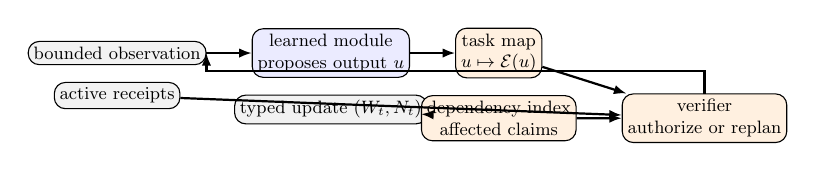
\begin{tikzpicture}[scale=0.72,transform shape,node distance=3mm and 8mm,
 box/.style={draw,rounded corners,align=center,inner sep=2.7pt,font=\small},
 learned/.style={box,fill=blue!8},symbolic/.style={box,fill=orange!12},
 data/.style={box,fill=gray!10},arr/.style={-{Latex[length=1.6mm]},thick}]
\node[data] (obs) {bounded observation};
\node[learned,right=of obs] (proposal) {learned module\\proposes output $u$};
\node[symbolic,right=of proposal] (obl) {task map\\$u\mapsto\mathcal E(u)$};
\node[data,below=of obs] (receipts) {active receipts};
\node[data,below=of proposal] (update) {typed update $(W_t,N_t)$};
\node[symbolic,below=of obl] (index) {dependency index\\affected claims};
\node[symbolic,right=of index] (decision) {verifier\\authorize or replan};
\draw[arr] (obs)--(proposal); \draw[arr] (proposal)--(obl);
\draw[arr] (receipts)--(decision); \draw[arr] (obl)--(decision);
\draw[arr] (update)--(index); \draw[arr] (index)--(decision);
\draw[arr] (decision.north) -- ++(0,4mm) -| (obs.east);
\end{tikzpicture}
\caption{Common runtime loop. In the graph task, $u$ is an answer and
$\mathcal E(u)$ contains three required edge claims. In RGB planning,
$u$ is an action and $\mathcal E(u)$ contains its required symbolic claims.
Policies, predicates, and learned weights are task-specific; the shared object is
the certificate-carrying interaction protocol.}
\label{fig:architecture}
\end{figure}

\section{Benchmark implementation}
\label{sec:method}

\subsection{Learned candidate ordering}

The Attribute scorer receives no numeric entity IDs or entity embeddings. Its two
MLP heads rank each supplied hop-specific candidate list from 31 observable coordinates:
acquired counts and weights, memory/frontier flags, within-list ranks,
budget state, semantic matches, and paid-probe statistics when available.  It is
trained only on source graphs for 20 epochs with AdamW at $3\times10^{-4}$.
Numeric-ID tie-breaking can still change visibility and rank-derived features;
complete features, loss, sample counts, and the relabeling counterexample are in
the supplement.

\subsection{Controller and trust boundary}

The fixed controller instantiates Eq.~\eqref{eq:query} as a query automaton. It
inspects the anchor, orders the visible middle nodes, traverses to a selected
middle node, inspects its successors, checks legal semantic claims, and
backtracks on failure. Learned scores only permute candidate lists; the controller
owns focus, action masking, budget, and the required-claim set. The general graph API
permits more actions than this automaton, so the reported protocol is defined by
controller $\mathcal K_\pi$ as well as API legality.

\section{Experimental design}
\label{sec:experiments}

\paragraph{Data.}
We construct compact neuron-level KGs from official releases and exclude raw EM
imagery, skeletons, meshes, and per-synapse point tables; the supplement reports
the exact node and edge counts by relation type.  H01 annotations are
official cortical-layer labels sampled at soma centroids.  MANC retains neurons
with a non-null curated \texttt{mancType}; HemiBrain retains traced, uncropped
neurons exported through neuPrint \citep{clements2020neuprint}.  Inverse wiring
edges are materialized.  We use publicly released datasets under their respective research licenses; the
supplement records source versions and access metadata.


\paragraph{First-page target prevalence.}
Define the \emph{first-page two-hop candidate union}
\[
 X^{\mathrm{fp}}_{d,V}(a)=\{x\in\mathcal V_d:\exists m,\
 (a,p,m)\in\Vis_{d,p,V}(a),\
 (m,p,x)\in\Vis_{d,p,V}(m)\}.
\]
This set is computed offline by opening the first continuation page for every
middle node disclosed on the anchor's first page. It is a dataset diagnostic,
not an agent observation, and no evaluated policy receives it. For query
$(a,y)$, its visible target prevalence is
\[
 s_{d,V}(a,y)=
 \frac{|A_d(a,y)\cap X^{\mathrm{fp}}_{d,V}(a)|}
 {\max\{1,|X^{\mathrm{fp}}_{d,V}(a)|\}}.
\]
A smaller value means that the target selects a smaller fraction of this
offline candidate union. Target counts and answer-set sizes are accompanying
statistics, not alternative definitions. Test queries use all seven H01 layer
targets, 1,945 MANC type targets among 3,893 graph types, and 2,278 HemiBrain
type targets among 5,554 graph types. Mean answer-set sizes are 45.5, 7.3, and
20.7, respectively. Cross-graph differences also include topology, weights,
and annotation coverage; we do not attribute them to target prevalence alone.




\paragraph{Splits and evaluation blocks.}
Neuron anchors are assigned to train, validation, or test by seeded cryptographic
hash; semantic targets are shared ontology nodes, not held-out neurons. For each
leave-one-connectome-out direction, the Attribute and Recurrent policies
train on the other two graphs with seeds 17, 29, and 43 and receive no entity
embeddings. Hyperparameters and selector checkpoints use source validation only.

The main comparison is the prospectively frozen held-out-pair evaluation in
Table~\ref{tab:fresh-test}. It holds the query automaton, visibility operator,
budget, action restrictions, verifier, and query set fixed while changing only
candidate ordering. Its controller ranks the complete visible first-hop frontier
without a paid probe. The 5,000-pair target-coarsening block holds the anchor, wiring, visibility
rule, controller, policy checkpoint, and random seed fixed while replacing only
the target predicate; because that predicate changes the query, subsequent
actions may differ. This is an explicitly exploratory mechanism audit.

\paragraph{Baselines and statistical unit.}
All main-table policies use observable information only. Random applies a
deterministic permutation keyed by run seed, query ID, current node, and candidate
ID. The Recurrent baseline uses the same 31 observed features and
source-graph decision snapshots as the Attribute scorer, but trains an LSTM ranker
with REINFORCE; its state resets at each ranking call. It is therefore an
access-matched recurrent control, not a reproduction of full-graph MINERVA.
The supplement gives architectures, training volumes, and hyperparameters.

Certificate success is averaged over 1,000 fixed query IDs and, for stochastic
policies, three fixed training/action seeds. After an audit found repeated first
anchors, we replaced query-wise resampling by a paired cluster bootstrap; this
post-outcome correction changes uncertainty estimates, not policies or point estimates. It first
averages seed outcomes within query, then resamples first-anchor clusters 10,000
times and retains every query in each sampled cluster. H01 has 837 clusters,
MANC 807, and HemiBrain 806 (maximum cluster size four). The two planned
fly-graph contrasts between Expert selector and Weight use Bonferroni-adjusted 97.5\%
intervals. H01 and all other contrasts are descriptive. The correction accounts
for repeated anchors but remains conditional on fitted checkpoints, fixed seeds,
the controller, and these graphs.




\section{Results}
\label{sec:results}

\subsection{Held-out evaluation under fixed access}

We fixed the controller, page size $V=32$, budget and horizon $B=H=64$,
candidate cap, policy checkpoints, and two fly-graph comparisons before
evaluating 1,000 previously unused query pairs per graph.  The queries share no
anchor--target pair with earlier evaluation sets.  Because first anchors repeat,
confidence intervals resample first-anchor clusters.  The three action/model
seeds are fixed computational replications; the intervals are conditional on
these seeds and on this query population.

Weight orders candidates by observed synaptic weight. Random uses a
query- and seed-keyed random permutation. Recurrent is an access-matched LSTM policy trained with REINFORCE. Attribute is the two-head
listwise MLP in Section~\ref{sec:method}. Expert selector chooses one
of the observable policies from source-graph features before acting.
Random$\rightarrow$Attribute randomizes only the first hop and uses Attribute
ordering at the second. Every policy receives the same observations, action
costs, and certificate-verification rule.
\begin{table}[h]
\centering\scriptsize
\setlength{\tabcolsep}{3pt}
\caption{Prospectively frozen evaluation on 1,000 previously unused query pairs per graph. Entries are certificate success/unconditional charged actions, averaged across seeds 17/29/43 for stochastic policies; Weight is deterministic. All policies use the same frozen controller and observations.}
\label{tab:fresh-test}
\begin{tabular}{lrrrrrr}
\toprule
Graph & Weight & Random & Recurrent & Attribute & Expert selector & Random$\to$Attribute \\
\midrule
H01 & 0.4090/42.63 & 0.5100/39.82 & 0.4840/40.64 & 0.4117/41.27 & 0.3920/43.14 & 0.4017/42.05 \\
MANC & 0.0990/60.18 & 0.1050/60.11 & 0.1030/60.01 & 0.1107/59.96 & 0.1120/60.03 & 0.1003/60.19 \\
HemiBrain & 0.1270/59.52 & 0.1347/59.23 & 0.1437/58.86 & 0.1343/58.91 & 0.1483/58.83 & 0.1367/58.86 \\
\bottomrule
\end{tabular}
\end{table}


No policy dominates on all three graphs.  Relative to Weight, Expert selector
changes certificate success by $+0.0213$ on HemiBrain (two-comparison
Bonferroni 95\% interval $[0.0030,0.0397]$), $+0.0130$ on MANC
($[-0.0094,0.0360]$), and $-0.0170$ on H01 (descriptive nominal interval
$[-0.0295,-0.0048]$). Random is strongest on H01, whereas Expert selector is
strongest on HemiBrain. A matched hop-attribution audit shows that replacing
the selector's first hop by Weight leaves all 9,000 outcomes unchanged. Thus the
observed HemiBrain difference is attributable to second-hop ordering, not to the
first-hop selector. Accordingly, the selector is an evaluated component rather than the primary
contribution.

Raw action means can reward early failure.  Outcome-conditioned aggregation
shows the opposite: unsuccessful episodes average about 51 charged actions on
H01 and 63 on MANC and HemiBrain. The controller reaches its 63-action
exploration limit in 29--37\% of H01 episodes, 89--90\% of MANC episodes, and
85--87\% of HemiBrain episodes. The supplement gives every policy;
these data identify acquisition exhaustion rather than low-cost failure.

\subsection{Target granularity controls acquisition difficulty}

Let $Y_d$ be the native target set and
$\bar Y_d=\{\bar y_1,\ldots,\bar y_7\}$ a disjoint set of synthetic coarse
targets. A fixed map $g_d:Y_d\to\bar Y_d$ replaces each semantic edge
$(x,\rho_d,y)$ by $(x,\bar\rho_d,g_d(y))$.  Consequently
$A_d(a,y)\subseteq\bar A_d(a,g_d(y))$.  This set inclusion is elementary; the
experiment measures its effect on paired anchors under a fixed visibility rule,
controller, policy checkpoint, and random tape. The target predicate, and hence
the realized actions, may differ.

We apply the transformation to 5,000 paired MANC and HemiBrain instances while
holding wiring, anchor, pairing identifier, policy checkpoint, and random seed
fixed.
\begin{table}[h]
\centering\scriptsize
\setlength{\tabcolsep}{3pt}
\caption{Paired label-coarsening audit, 5,000 original native queries per fly graph. Every entry is native/coarse. Visible target prevalence is the relevant fraction among first-page two-hop candidate nodes; other columns are Success$(64)$, averaged over the original action/model seeds. No new model fitting.}
\label{tab:ladder}
\begin{tabular}{lrrrr}
\toprule
Graph & \shortstack{Visible target\\prevalence} & Weight & Random & Attribute \\
\midrule
MANC & 0.0060/0.1476 & 0.0972/0.8226 & 0.1093/0.9036 & 0.1088/0.8644 \\
HemiBrain & 0.0191/0.1535 & 0.1290/0.7858 & 0.1765/0.8887 & 0.1373/0.8167 \\
\bottomrule
\end{tabular}
\end{table}

Visible target prevalence increases from $0.0060$ to $0.1476$ on MANC and from
$0.0191$ to $0.1535$ on HemiBrain; success rises substantially for all three
reported policies. Thus semantic target granularity materially changes acquisition difficulty in
this controlled intervention; it is not evidence that one ordering algorithm
alone solves the native regime. A privileged visible-witness ordering solves every generated query
within 16 actions, confirming that the gap is observable acquisition rather than
answer non-existence.




\subsection{Certificate verification}

The policy-independent standard-library verifier sees the public query, proposed witness,
certificate, and trusted issuance context, but no graph or answer set. It
accepts all \VerifierReplayCertificates{} unmodified nonempty submissions from
\VerifierReplayEpisodes{} graph-search episodes; empty submissions are not
certificates. In a separate diagnostic it rejects all
\VerifierMutationAttempts{} constructed binding and structural mutations. This
tests policy-independent logical support under a trusted issuer, not search
quality or an attack-rate bound; class-by-graph counts and the trusted-registry
assumption are in the supplement.

\section{RGB semantic-map evaluation}
\label{sec:route-memory}


BabyAI UnlockPickupDist \citep{chevalierboisvert2023minigrid} instantiates the
same claim--receipt--certificate interface. Every method receives the same
egocentric $7\times7$ RGB image, position relative to the initial pose, exact
cardinal direction, inventory type, mission string, and last-action outcome. A
frozen tile classifier converts the RGB image into semantic-map claims, each
linked to the corresponding immutable image receipt. For a proposed action
$a$, $\mathcal E_t(a)$ is its finite set of required symbolic claims.
Authorization requires active receipt support for every claim in
$\mathcal E_t(a)$. A receipt proves image acquisition, not the physical truth
of the learned interpretation.


\paragraph{Dependency-indexed plan validation.}
Let $\mathcal I$ be the receipt-identifier set and $\mathcal K$ the set of
semantic update keys.  At decision time $t$, the deterministic planner's
retained suffix is $\Pi_t=(a_{c_t},\ldots,a_L)$.  Let $A_t\subseteq\mathcal I$
be the active receipts and let $\theta_t$ be the current semantic-key valuation.
For every $i\ge c_t$, define
$\operatorname{Supp}_i(A_t,\theta_t)\in\{0,1\}$ to indicate whether every
required claim of $a_i$ has support from an active receipt.

The recorded set $D_i\subseteq\mathcal I$ is \emph{receipt-complete} when the
following implication holds for all $A,A'$ and $\theta$: if $A$ and $A'$ differ
only in receipt $r$ and $\operatorname{Supp}_i(A,\theta)\ne
\operatorname{Supp}_i(A',\theta)$, then $r\in D_i$. The recorded set
$K_i\subseteq\mathcal K$ is \emph{key-complete} when it contains every
semantic key whose value is read either by $\operatorname{Supp}_i$ or by the
planner when constructing $a_i$ and its required-claim set. A changed key in
$K_i$ therefore marks the retained suffix stale even if its currently cached
support value remains one.
For an update from $(A_t,\theta_t)$ to $(A_{t+1},\theta_{t+1})$, let
$W_t=A_t\mathbin{\triangle}A_{t+1}$ and let $N_t$ contain exactly the keys
whose values changed; write $\Delta_t=(W_t,N_t)$. The affected positions are
\[
 \mathcal J(\Delta_t)=\{i\ge c_t:D_i\cap W_t\ne\varnothing
 \ \text{or}\ K_i\cap N_t\ne\varnothing\}.
\]
The dependency index stores the exact inverse maps
$L_{\mathcal I}(r)=\{i:r\in D_i\}$ and
$L_{\mathcal K}(k)=\{i:k\in K_i\}$.

\begin{proposition}[Coverage and authorization]\label{prop:receipt-support}
If $D_i$ is receipt-complete, $K_i$ is key-complete, and both inverse maps are
exact, then $\mathcal J(\Delta_t)$ contains every suffix position whose support
value changes and every position whose recorded planner-read key changes.
Consequently, a controller that revalidates those positions, replans after a
recorded planner-read change, and authorizes the next action only with current
support never authorizes that checked action after its final active support is
withdrawn. The conclusion is relative to the trusted issuer and symbolic
action model; it does not establish physical correctness.
\end{proposition}

\begin{proposition}[Selective-validation equivalence]
\label{prop:receipt-next-action}
Suppose complete suffix validation and dependency-indexed validation receive
the same retained suffix, active receipts, semantic valuation, update, and
deterministic planner, and an exact cached pre-update support vector.
Both procedures use the same retention rule: retain exactly when all
post-update support values equal one and
$N_t\cap\bigcup_{i=c_t}^{L}K_i=\varnothing$; otherwise invoke the common
planner. Under the completeness assumptions of
Proposition~\ref{prop:receipt-support}, they therefore return the same next
authorization decision. This statement does not compare either procedure with
eager replanning after a change outside the recorded read dependencies that
could make an unrelated alternative plan preferable.
\end{proposition}

\begin{corollary}[Amortized location work]
\label{cor:receipt-location-work}
Within one retained-plan epoch with fixed cursor $c$, let
$Z=\sum_{i=c}^{L}(|D_i|+|K_i|)$ at index construction. With
expected-constant-time hash lookup, construction followed by $M$ updates has
location work
\[
 O\!\left(Z+\sum_{t=1}^{M}\left[|W_t|+|N_t|
 +\sum_{r\in W_t}|L_{\mathcal I}(r)|
 +\sum_{k\in N_t}|L_{\mathcal K}(k)|\right]\right).
\]
Complete suffix validation instead visits $M(L-c+1)$ positions. Across multiple
retained-plan epochs, both costs sum over epochs. Predicate checks, index
maintenance, and planning after rejection are additional costs and are
reported separately in the experiment.
\end{corollary}



We compare full replanning, complete validation of the retained plan,
dependency-indexed validation, and unchecked reuse under the same planner,
action model, RGB observations, and generated update schedule. The study
generated 800 layouts and retained 513 by a method-independent eligibility rule,
yielding 12,312 method--condition rows and 3,078 complete paired cells. Every
stored environment trace replays exactly.


\begin{figure*}[t]
\centering
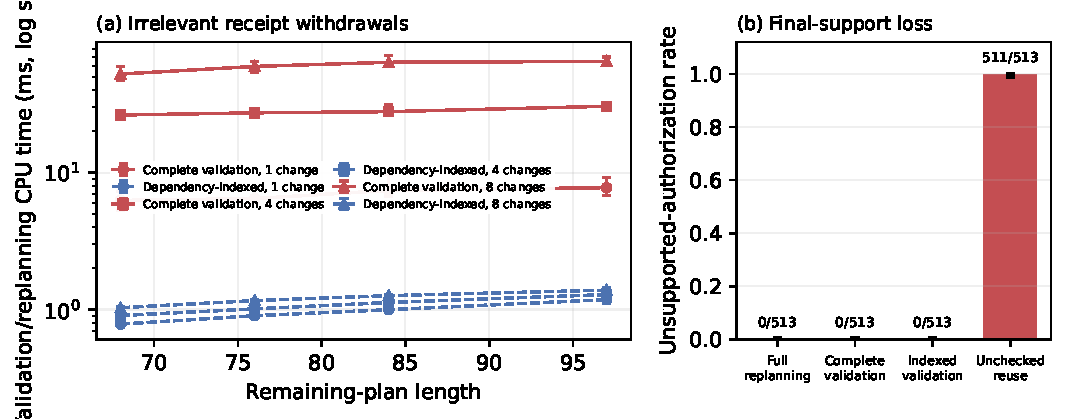
\includegraphics[width=\textwidth]{generated/revalidation_tradeoff.pdf}
\caption{Two distinct interventions under matched RGB access. (a) In the
primary long-plan population with four or eight irrelevant receipt withdrawals,
dependency-indexed and complete retained-plan validation agree on all
\AmortizedPairedCells{} paired decisions, while indexing reduces
validation-and-replanning CPU time by \AmortizedReduction{} (layout-bootstrap 95\% interval
[\AmortizedReductionLow{}, \AmortizedReductionHigh{}]); curves also show the
one-withdrawal condition descriptively. (b) After final-support loss, every
checking method prevents unsupported authorization, whereas unchecked reuse
does not. Binomial bars are exact 95\% intervals.}
\label{fig:selective-validation}
\end{figure*}



The prospectively frozen primary population contains \AmortizedEligible{}
layouts with at least 64 remaining actions and four or eight distinct irrelevant
receipt withdrawals, yielding \AmortizedPairedCells{} paired timing cells.
Dependency-indexed and complete retained-plan validation agree on
\AmortizedAgreement{} of authorization decisions. We define
\emph{validation-and-replanning CPU time} as index construction, index
maintenance, required-claim validation, and planner calls; it excludes CNN
inference, simulator stepping, and action execution. Dependency indexing reduces
this endpoint by \AmortizedReduction{} relative to complete validation (layout-bootstrap 95\% interval
[\AmortizedReductionLow{}, \AmortizedReductionHigh{}]). Panel~(a) additionally
shows the prospectively specified one-update condition descriptively.

In a separate final-support-loss intervention, full replanning, complete
validation, and dependency-indexed validation make zero unsupported
authorizations in 513 episodes; unchecked reuse makes 511. Thus the efficiency
result concerns sparse irrelevant changes, while the safety result tests removal
of the final support for the current action. Neither comparison asserts an
advantage in physical action count or perception accuracy.





\section{Discussion}

The experiments establish three separable facts. First, target granularity and the resulting visible target prevalence strongly
affect witness acquisition under fixed wiring, visibility, and action budgets. Second, no candidate ordering is uniformly best: random branch
diversification is competitive on two graphs, while learned second-hop ordering
helps on HemiBrain. Third, certificate validity is independent of search quality.
A weak policy may return no certificate; a successful policy is accepted only
when its active receipts support every required claim.

The RGB instantiation isolates a control mechanism rather than a broad robotics
result. On long retained plans with repeated sparse updates, dependency indexing
preserves the decisions of complete retained-plan validation while reducing
validation-and-replanning CPU time, including index construction and
maintenance.
Unchecked reuse demonstrates the corresponding safety failure after final
support loss.
The RGB study evaluates evidence management rather than comparative performance
against model-free reinforcement learning, physical action efficiency, or the
correctness of learned perception. Only the
interface transfers between graph exploration and RGB planning; policies,
planners, and required-claim definitions remain task-specific.

These guarantees assume a trusted issuer, complete dependencies, and declared
update semantics; they neither authenticate receipts nor detect a wrong issuer.
The validation procedures are equivalent only under
Proposition~\ref{prop:receipt-next-action} and need not match global replanning
after unrelated changes. \href{https://anonymous.4open.science/r/connectomequest/README.md}{Anonymous code and artifacts}.



\clearpage
\bibliographystyle{plainnat}
\bibliography{references}

\end{document}
